%%%% old figures for valr manuscript %%%%

%%%%%%%%%%%% Previous Figures %%%%%%%%%%%


%%%% TSS H3K4me3 example %%%%
\begin{figure}
\centering
    \begin{subfigure}[b]{0.45\textwidth}
\begin{Shaded}
\begin{Highlighting}[]
\NormalTok{x <-}\StringTok{ }\KeywordTok{trbl_interval}\NormalTok{(}
  \NormalTok{~chrom, ~start, ~end,}
  \StringTok{'chr1'}\NormalTok{, }\DecValTok{25}\NormalTok{,     }\DecValTok{50}\NormalTok{,}
  \StringTok{'chr1'}\NormalTok{, }\DecValTok{100}\NormalTok{,    }\DecValTok{125}
\NormalTok{)}

\NormalTok{y <-}\StringTok{ }\KeywordTok{trbl_interval}\NormalTok{(}
  \NormalTok{~chrom, ~start, ~end,}
  \StringTok{'chr1'}\NormalTok{, }\DecValTok{30}\NormalTok{,     }\DecValTok{75}
\NormalTok{)}

\KeywordTok{bed_glyph}\NormalTok{(}\KeywordTok{bed_intersect}\NormalTok{(x, y))}
\end{Highlighting}
\end{Shaded}
        \label{fig:bed_glyph_code}
    \end{subfigure}
    ~
\begin{subfigure}[b]{0.45\textwidth}
        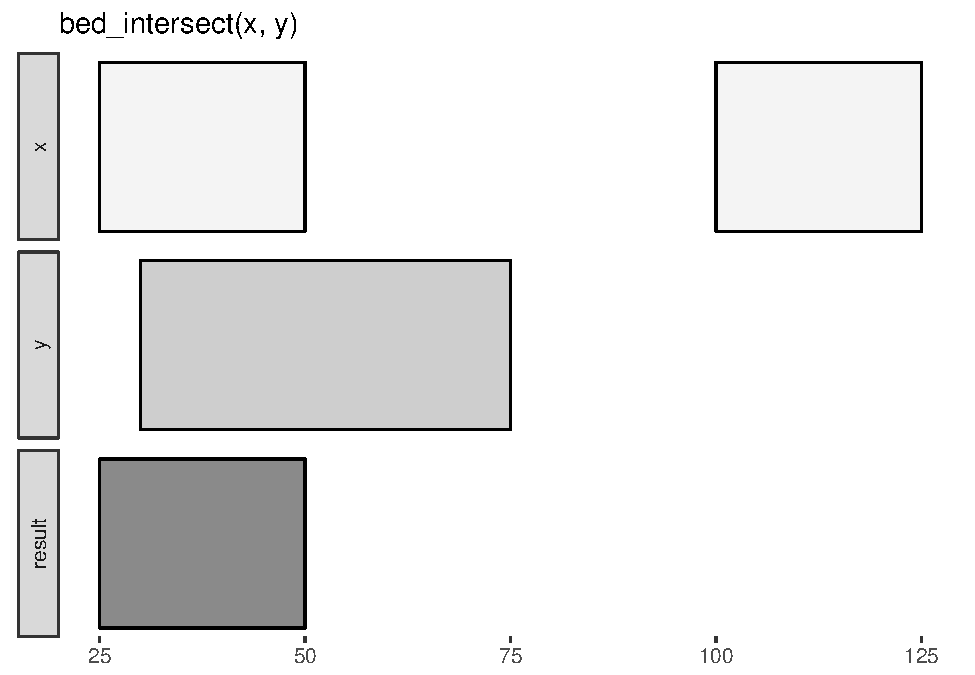
\includegraphics[width=\textwidth]{intersect_glyph-1.pdf}
        \label{fig:bed_glyph_out}
    \end{subfigure}
\caption{\label{fig:your-figure}Visualizing interval intersections with valr.	 }
\end{figure}

\begin{figure}
\centering
    \begin{subfigure}[b]{\textwidth}
\begin{Shaded}
\begin{Highlighting}[]
\CommentTok{# `valr_example()` identifies the path of example files}
\NormalTok{bedfile <-}\StringTok{ }\KeywordTok{valr_example}\NormalTok{(}\StringTok{'genes.hg19.chr22.bed.gz'}\NormalTok{)}
\NormalTok{genomefile <-}\StringTok{ }\KeywordTok{valr_example}\NormalTok{(}\StringTok{'hg19.chrom.sizes.gz'}\NormalTok{)}
\NormalTok{bgfile  <-}\StringTok{ }\KeywordTok{valr_example}\NormalTok{(}\StringTok{'hela.h3k4.chip.bg.gz'}\NormalTok{)}

\NormalTok{genes <-}\StringTok{ }\KeywordTok{read_bed}\NormalTok{(bedfile, }\DataTypeTok{n_fields =} \DecValTok{6}\NormalTok{)}
\NormalTok{genome <-}\StringTok{ }\KeywordTok{read_genome}\NormalTok{(genomefile)}
\NormalTok{y <-}\StringTok{ }\KeywordTok{read_bedgraph}\NormalTok{(bgfile)}

\CommentTok{# generate 1 bp TSS intervals, `+` strand only}
\NormalTok{tss <-}\StringTok{ }\NormalTok{genes %>%}\StringTok{ }\KeywordTok{filter}\NormalTok{(strand ==}\StringTok{ '+'}\NormalTok{) %>%}\StringTok{ }\KeywordTok{mutate}\NormalTok{(}\DataTypeTok{end =} \NormalTok{start +}\StringTok{ }\DecValTok{1}\NormalTok{)}

\CommentTok{# 1000 bp up and downstream}
\NormalTok{region_size <-}\StringTok{ }\DecValTok{1000}

\CommentTok{# 50 bp windows}
\NormalTok{win_size <-}\StringTok{ }\DecValTok{50}

\CommentTok{# add slop to the TSS, break into windows and add a group}
\NormalTok{x <-}\StringTok{ }\NormalTok{tss %>%}\StringTok{ }\KeywordTok{bed_slop}\NormalTok{(genome, }\DataTypeTok{both =} \NormalTok{region_size) %>%}
\StringTok{  }\KeywordTok{bed_makewindows}\NormalTok{(genome, win_size)}

\CommentTok{# map signals to TSS regions and calculate summary statistics.}
\NormalTok{res <-}\StringTok{ }\KeywordTok{bed_map}\NormalTok{(x, y, }\DataTypeTok{win_sum =} \KeywordTok{sum}\NormalTok{(value, }\DataTypeTok{na.rm =} \OtherTok{TRUE}\NormalTok{)) %>%}
\StringTok{  }\KeywordTok{group_by}\NormalTok{(.win_id) %>%}
\StringTok{  }\KeywordTok{summarize}\NormalTok{(}\DataTypeTok{win_mean =} \KeywordTok{mean}\NormalTok{(win_sum, }\DataTypeTok{na.rm =} \OtherTok{TRUE}\NormalTok{),}
            \DataTypeTok{win_sd =} \KeywordTok{sd}\NormalTok{(win_sum, }\DataTypeTok{na.rm =} \OtherTok{TRUE}\NormalTok{))}

\NormalTok{x_labels <-}\StringTok{ }\KeywordTok{seq}\NormalTok{(-region_size, region_size, }\DataTypeTok{by =} \NormalTok{win_size *}\StringTok{ }\DecValTok{5}\NormalTok{)}
\NormalTok{x_breaks <-}\StringTok{ }\KeywordTok{seq}\NormalTok{(}\DecValTok{1}\NormalTok{, }\DecValTok{41}\NormalTok{, }\DataTypeTok{by =} \DecValTok{5}\NormalTok{)}

\NormalTok{sd_limits <-}\StringTok{ }\KeywordTok{aes}\NormalTok{(}\DataTypeTok{ymax =} \NormalTok{win_mean +}\StringTok{ }\NormalTok{win_sd, }\DataTypeTok{ymin =} \NormalTok{win_mean -}\StringTok{ }\NormalTok{win_sd)}

\KeywordTok{ggplot}\NormalTok{(res, }\KeywordTok{aes}\NormalTok{(}\DataTypeTok{x =} \NormalTok{.win_id, }\DataTypeTok{y =} \NormalTok{win_mean)) +}\StringTok{ }\KeywordTok{geom_point}\NormalTok{() +}\StringTok{ }\KeywordTok{ylab}\NormalTok{(}\StringTok{'Signal'}\NormalTok{) +}
\StringTok{  }\KeywordTok{scale_x_continuous}\NormalTok{(}\DataTypeTok{labels =} \NormalTok{x_labels, }\DataTypeTok{breaks =} \NormalTok{x_breaks) +}\StringTok{ }
\StringTok{  }\KeywordTok{ggtitle}\NormalTok{(}\StringTok{'Human H3K4me3 signal near transcription start sites'}\NormalTok{) +}
\StringTok{  }\KeywordTok{xlab}\NormalTok{(}\StringTok{'Position (bp from TSS)'}\NormalTok{) +}\StringTok{ }\KeywordTok{geom_pointrange}\NormalTok{(sd_limits) +}
\StringTok{  }\KeywordTok{theme_classic}\NormalTok{()}
\end{Highlighting}
\end{Shaded}
        \label{fig:meta_gene_code}
    \end{subfigure}

\begin{subfigure}[b]{0.5\textwidth}
        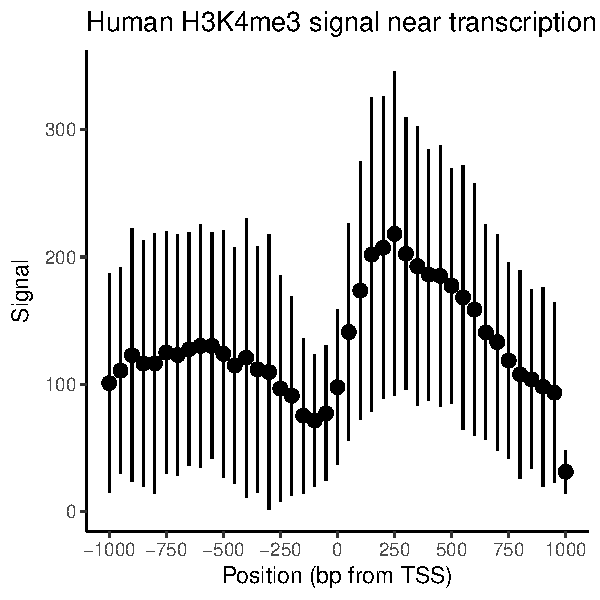
\includegraphics[width=\textwidth]{demo-tss-1.pdf}
        \label{fig:meta_gene_out}
    \end{subfigure}
\caption{\label{fig:your-figure}Meta-analysis of signals relative to genomic features with valr.}
\end{figure}


%%%% DNA methylation example %%%%

\subsection{Get the public datasets from
UCSC}\label{get-the-public-datasets-from-ucsc}

\begin{Shaded}
\begin{Highlighting}[]
\KeywordTok{library}\NormalTok{(dplyr)}
\KeywordTok{library}\NormalTok{(valr)}
\KeywordTok{library}\NormalTok{(R.utils)}
\KeywordTok{library}\NormalTok{(curl)}
\KeywordTok{library}\NormalTok{(ggplot2)}
\KeywordTok{library}\NormalTok{(gridExtra)}
\end{Highlighting}
\end{Shaded}

\begin{Shaded}
\begin{Highlighting}[]
\NormalTok{DMSO_treated<-}\KeywordTok{read_bed}\NormalTok{(}\StringTok{'http://hgdownload.soe.ucsc.edu/goldenPath/hg19/encodeDCC/wgEncodeHaibMethylRrbs/wgEncodeHaibMethylRrbsA549Dm002p7dHaibSitesRep1.bed.gz'}\NormalTok{, }\DataTypeTok{n_fields=}\DecValTok{6}\NormalTok{, }\DataTypeTok{skip=}\DecValTok{1}\NormalTok{)}
\end{Highlighting}
\end{Shaded}

\begin{Shaded}
\begin{Highlighting}[]
\NormalTok{untreated<-}\KeywordTok{read_bed}\NormalTok{(}\StringTok{'http://hgdownload.soe.ucsc.edu/goldenPath/hg19/encodeDCC/wgEncodeHaibMethylRrbs/wgEncodeHaibMethylRrbsAg04449UwSitesRep1.bed.gz'}\NormalTok{, }\DataTypeTok{n_fields=}\DecValTok{6}\NormalTok{, }\DataTypeTok{skip=}\DecValTok{1}\NormalTok{)}
\end{Highlighting}
\end{Shaded}

To view the data

\begin{Shaded}
\begin{Highlighting}[]
\KeywordTok{head}\NormalTok{(untreated)}
\end{Highlighting}
\end{Shaded}

\begin{verbatim}
#> # A tibble: 6 x 6
#>   chrom start   end           name score strand
#>   <chr> <int> <int>          <chr> <chr>  <chr>
#> 1  chr1 10785 10786 AG04449_0__JS_     1      +
#> 2  chr1 10788 10789 AG04449_0__JS_     1      +
#> 3  chr1 10794 10795 AG04449_0__JS_     1      +
#> 4  chr1 10810 10811 AG04449_0__JS_     1      +
#> 5  chr1 10812 10813 AG04449_0__JS_     1      +
#> 6  chr1 10815 10816 AG04449_0__JS_     1      +
\end{verbatim}

\subsection{Examine regions that are different and regions that
intersect}\label{examine-regions-that-are-different-and-regions-that-intersect}

\begin{Shaded}
\begin{Highlighting}[]
\NormalTok{different_region<-}\KeywordTok{bed_subtract}\NormalTok{(DMSO_treated,untreated, }\DataTypeTok{any=}\OtherTok{FALSE}\NormalTok{)}
\KeywordTok{dim}\NormalTok{(different_region)}
\end{Highlighting}
\end{Shaded}

\begin{verbatim}
#> [1] 278241      6
\end{verbatim}

\begin{Shaded}
\begin{Highlighting}[]
\NormalTok{intersect_region<-}\KeywordTok{bed_intersect}\NormalTok{(DMSO_treated,untreated, }\DataTypeTok{suffix=}\KeywordTok{c}\NormalTok{(}\StringTok{'.treated'}\NormalTok{,}\StringTok{'.untreated'}\NormalTok{))}
\KeywordTok{dim}\NormalTok{(intersect_region)}
\end{Highlighting}
\end{Shaded}

\begin{verbatim}
#> [1] 1576400      12
\end{verbatim}

\subsection{Plot the distribution of different regions and intersected
regions across
chromosomes}\label{plot-the-distribution-of-different-regions-and-intersected-regions-across-chromosomes}

\begin{Shaded}
\begin{Highlighting}[]
\NormalTok{p1<-}\KeywordTok{ggplot}\NormalTok{(}\DataTypeTok{data=}\NormalTok{different_region, }\KeywordTok{aes}\NormalTok{(}\DataTypeTok{x=}\NormalTok{chrom))+}\KeywordTok{geom_histogram}\NormalTok{(}\DataTypeTok{stat=}\StringTok{'count'}\NormalTok{, }\KeywordTok{aes}\NormalTok{(}\KeywordTok{factor}\NormalTok{(chrom), }\DataTypeTok{fill=}\StringTok{'differential methylation'}\NormalTok{))+}\KeywordTok{scale_fill_brewer}\NormalTok{(}\DataTypeTok{palette =} \StringTok{'Set2'}\NormalTok{)+}\KeywordTok{theme_minimal}\NormalTok{()+}\KeywordTok{ggtitle}\NormalTok{(}\StringTok{'Distribution of differential methylation across chromosomes'}\NormalTok{)+}\KeywordTok{theme}\NormalTok{(}\DataTypeTok{axis.text.x =} \KeywordTok{element_text}\NormalTok{(}\DataTypeTok{angle =} \DecValTok{45}\NormalTok{, }\DataTypeTok{hjust =} \DecValTok{1}\NormalTok{))}
\end{Highlighting}
\end{Shaded}

\begin{verbatim}
#> Warning: Ignoring unknown parameters: binwidth, bins, pad
\end{verbatim}

\begin{Shaded}
\begin{Highlighting}[]
\NormalTok{p2<-}\KeywordTok{ggplot}\NormalTok{(}\DataTypeTok{data=}\NormalTok{intersect_region, }\KeywordTok{aes}\NormalTok{(}\DataTypeTok{x=}\NormalTok{chrom))+}\KeywordTok{geom_histogram}\NormalTok{(}\DataTypeTok{stat=}\StringTok{'count'}\NormalTok{, }\KeywordTok{aes}\NormalTok{(}\KeywordTok{factor}\NormalTok{(chrom), }\DataTypeTok{fill=}\StringTok{'overlap methylation'}\NormalTok{))+}\KeywordTok{scale_fill_brewer}\NormalTok{(}\DataTypeTok{palette =} \StringTok{'Spectral'}\NormalTok{)+}\KeywordTok{theme_minimal}\NormalTok{()+}\KeywordTok{ggtitle}\NormalTok{(}\StringTok{'Distribution of overlapping methylation across chromosomes'}\NormalTok{)+}\KeywordTok{theme}\NormalTok{(}\DataTypeTok{axis.text.x =} \KeywordTok{element_text}\NormalTok{(}\DataTypeTok{angle =} \DecValTok{45}\NormalTok{, }\DataTypeTok{hjust =} \DecValTok{1}\NormalTok{))}
\end{Highlighting}
\end{Shaded}

\begin{verbatim}
#> Warning: Ignoring unknown parameters: binwidth, bins, pad
\end{verbatim}

\begin{Shaded}
\begin{Highlighting}[]
\KeywordTok{grid.arrange}\NormalTok{(p1, p2, }\DataTypeTok{ncol =} \DecValTok{1}\NormalTok{, }\DataTypeTok{nrow =}\DecValTok{2}\NormalTok{)}
\end{Highlighting}
\end{Shaded}
\begin{figure}
\begin{center}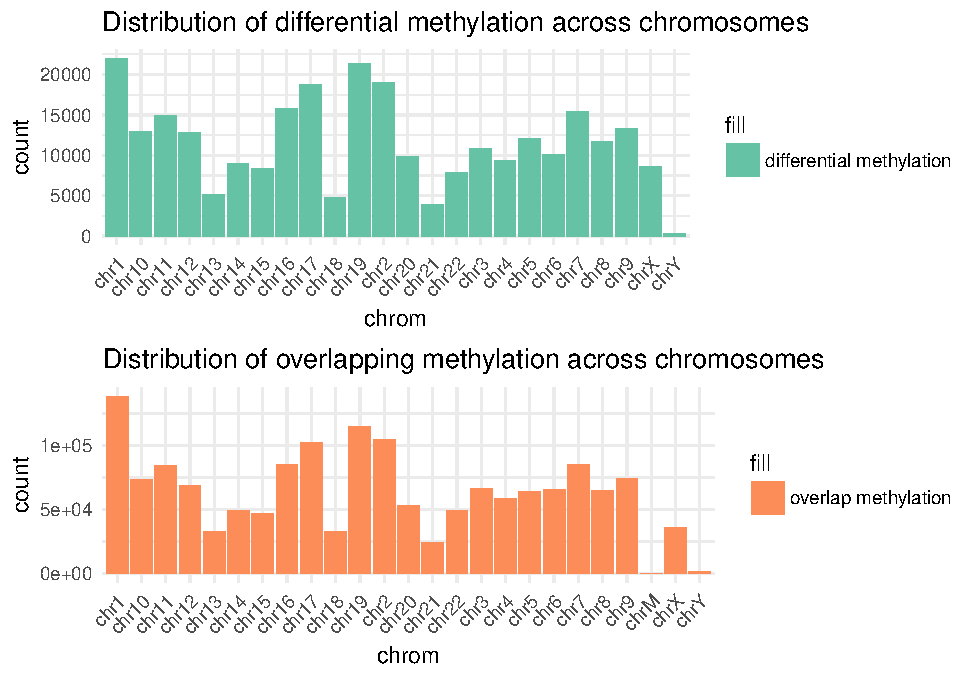
\includegraphics{unnamed-chunk-8-1} \end{center}
\end{figure}
